\setchapterpreamble[u]{\margintoc}
\chapter{Realtime Multi-Messenger Astronomy}
\labch{realtime}

In recent years, there has been a significant renewed interest in the study of transient and variable objects in astronomy. Driven primarily by the speed at which objects can evolve and disappear, particularly GRBs and latterly Kilonovae, it is often essential that astronomy can be done with minimal latency. In this vein, it is now commonplace for detectors to automatically issue so-called alerts for observations that meet given criteria, to enable other instruments to rapidly obtain near-simultaneous observations. Realtime alerts are automatically issued by GRB-searching instruments such as Swift-BAT and Fermi-GBM, while gravitaional-wave events are issued by the LIGO-VIRGO observatories, and high-energy neutrino alerts are issued by IceCube as well as ANTARES.

These alerts are all typically issued via  the Gamma-ray Coordination Network (GCN) system, where observatories can subscribe to automatically be notified or point.  An essential component of this process is the additional information published by astronomers, via GCN or Astronomers Telegrams (ATELs), in which follow-up observations are coordinated. There have been two high-profile examples of this, namely the comprehensive followup of GW170817/GRB170817A that led to the first unambiguous observation of a kilonovae, and the followup of high-energy neutrino IC170922A, which led to the identification of TXS 0506+056 as the first candidate source of TeV neutrinos. 

As part of this thesis, the author maintained and further developed the IceCube Realtime System from October 2018 onwards, acting as first responder to the vast majority of neutrino alerts in that period.

\section{The IceCube Realtime System}
The IceCube Realtime System has been operating since 2016, providing the first source of high-energy neutrino alerts. The first iteration of the alert system consisted of two streams, namely High-Energy Starting Events (HESE) and Extremely High Energy (EHE) events CITE. Each was an established event selection used to identify likely-astrophysical neutrinos cite. Filters to identify relevant events are deployed on computers at the South Pole, and detections are flagged  with low latency. After fast "online" reconstruction algorithms are applied to events, an automated machine-readable "notice" is distributed via the GCN system. In parallel, data from the event is transmitted via satellite to a computing centre in Madison, Wisconsin where a full likelihood scan is performed on the event (see chapter \ref{Event Selection and Reconstruction} for more details). 

Give V1 rates!

The alerts are vetted by humans to asses the event quality, with visually inspection being used to confirm classified topology and event reconstructions. The operating state of the detector is additionally checked. Following these steps, a plain-text GCN circular is distrubuted via the GCN system to confirm the good nature of the alert, and to provide the updated localisation arising from the full scan. 

This original system of alerts continued until May 2019, at which point a new alert system was implemented. While the original EHE selection was maintained, the HESE alert selection was improved to reduce the cascade contamination, and improve the astrophysical purity. In addition, a new alert stream based on the GFU event selection was initiated, with a significantly-elevated rate relative to EHE and HESE alerts. The publication of these three alert streams was unified into a new IceCube Astrotrack GCN stream, which was further subdivided into Gold and Bronze based on the average purity of alerts. Golden Astrotrack alerts will, as an ensemble, have an average of 50\% astrophysical neutrinos, while Bronze Astrotrack will have an average of 30\% astrophysical neutrinos.

A summary of all neutrino alerts issued to date is provided in table X. Individual neutrino alerts of interest are summarised in subsequent sections. 

\subsection{IC160427A - The "PanSTARRS Supernova Neutrino"}

The first alert issued under this system, HESE alert IC160427A, was found to be in spatial coincidence with an optical transient detected by the Pan-STARRS Observatory while following up the alert. This transient was initially tentaively classified as a Type Ic supernova, for which various models have predicted neutrino emission (see \ref{Neutrino Sources}).  However, the further spectroscopic and photometric evolution indicated that this was  more likely a Type Ia Supernova, for which no neutrino emission would be expected. Nonetheless, dedicated efforts to simulate an ensemble of IC160427A-like events led to the first characterisation of the impact of systematic uncertainties in modelling the polar glacial ice on directional reconstruction with IceCube for high-energy alerts. 

\subsection{IC170922A The "TXS 0506+056 Neutrino"}
Subsequent neutrino alerts did not yield any probable counterparts, until the detection of EHE alert IC170922A in spatial coincidence with flaring blazar TXS 0506+056. Chance coincidence in this case was estimated  This event was also resimulated in the same manner as IC160427A. Remarkably, despite its radically-different topology of through-going muon rather than starting track, the results were found to be broadly consistent. More details are given in chapter N.

\subsection{IC190331A - The "Multi-PEV Neutrino"}

A starting track was observed 

\subsection{IC190730A - The "PKS 1502+106 Neutrino"}

IC190730A was a golden neutrino alert with a signalness of roughly 65\%. Following the automated notice, Millipede Reconstruction clearly showed it was well-localised, and spatially coincident with blazar PKS 1502+106. This particular blazar is extremely bright, being Nth brightest in the sky in terms of integrated gamma-ray energy flux, and owing to its high redshift of z=1.xxx, is one of the most luminous known blazars. This coincidence was reported in the corresponding GCN circular, and triggered a broad multi-wavelength follow-up campaign. The archival SED is provided in figure N, originally from X, but annotated to illustrate contemporaneous observations from other instruments.

\begin{figure}[!ht]
	\centering 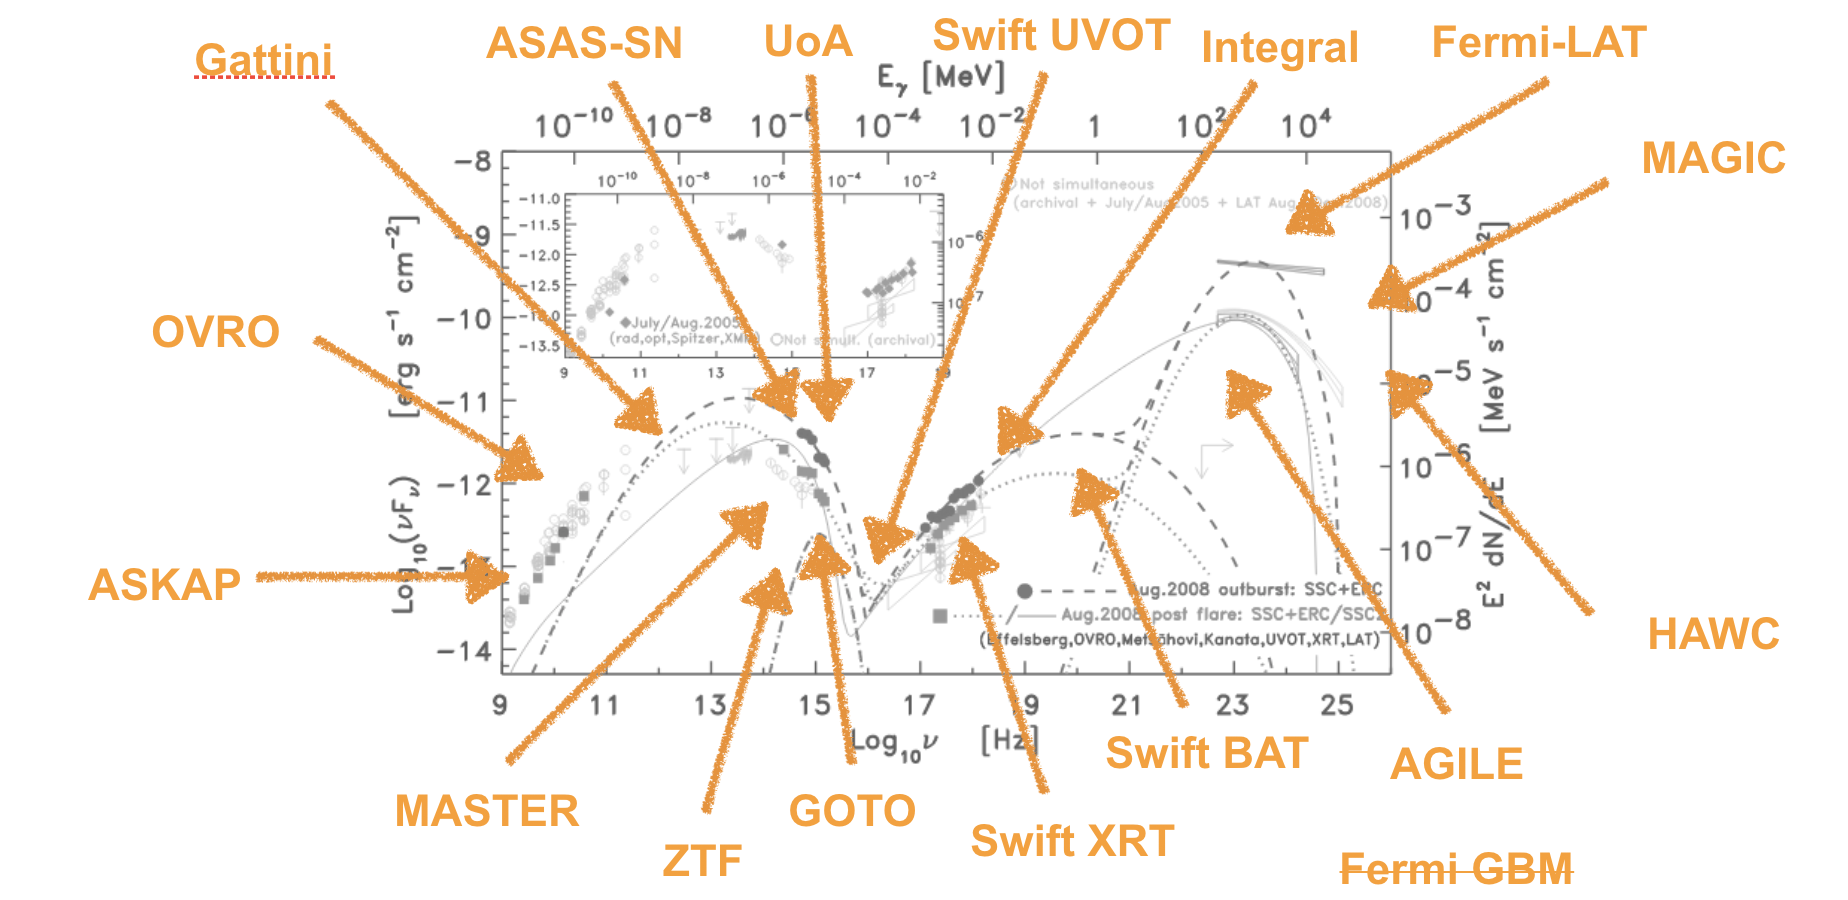
\includegraphics{pks_followup}
	\caption{The archival SED of PKS 1502+106 from X is shown. In orange, the names of various instruments that observed the source are shown, with orange arrows to indicate their corresponding energy regimes. CITEA-Z}
	\label{fig:PKSobs}
\end{figure}

Despite comprehensive wavelength coverage, 

The chance coincidence for at least one neutrino alert to be coincident with any of the  15 brightest blazars was calculated by the author, and found to be disfavoured at the level of 2.n sigma following the procedure in N. 

\subsection{IC190927A - The "SN2019xxx Neutrino"}

\subsection{IC191001A - The "Bran Stark Neutrino"}

\subsection{IC200107A - The "Flaring Extreme Blazar neutrino"}

\section{Interpreting high-energy neutrino alerts}

lalala

\subsection{Cluster searches}
lalaland

\subsection{OFU and GFU}.